\documentclass[]{article}

\usepackage{graphicx}
\usepackage{amssymb}
\usepackage{amsthm}
\usepackage{amsmath}
\usepackage{multirow}
\usepackage[section]{placeins}
\usepackage{hyperref}
\hypersetup{
	colorlinks,
	citecolor=black
	filecolor=black,
	linkcolor=blue,
	urlcolor=black
}
%opening
\title{EML6934 Midterm Exam}
\author{Elias Reyes}

\begin{document}

\maketitle

\begin{abstract}

\end{abstract}

\section{Differential Equations of Motion}
The equations of motion were derived using both Newton's second law and Lagrange's equations. The schematic for problem can be seen Figure \ref{fig:schematic}. The spacecraft is modeled as point \(P\) of  mass \(m\). The spacecraft moves relative to an inertial reference frame \(l\). The reference frame fixed in \(l\) is expressed as \(\{e_{x},e_{y},e_{z}\}\). The position of the spacecraft is denoted as \(r_{P/O}\), where \(O\) is modeled as the sun, fixed in \(l\). The spacecraft is parameterized in the basis \(\{u_{r},u_{\theta},u_{z}\}\), where the rotation is about \(u_{z}\) = \(e_{z}\). The rotation creates an angle \(\theta\) between \(e_{x}\) and \(u_{r}\), which can be seen in Figure \ref{fig:rotation2}.

\begin{figure}
	\centering
    \includegraphics[width=85mm,scale=0.85]{midterm_schematic.png}
	\caption{Schematic of particle moving in an inertially fixed plane}
	\label{fig:schematic}
\end{figure}
\begin{figure}
	\centering
	\includegraphics[width=75mm,scale=0.75]{rotation.png}
	\caption{Reference frame rotation}
	\label{fig:rotation2}
\end{figure}
Two forces are said to act on the spacecraft. The first is the gravitational force which is given as
\begin{equation} \label{grav_force}
	G = -m\mu\frac{r_{P/O}}{||r_{P/O}||^3},
\end{equation}
%\[G = -m\mu\frac{r_{P/O}}{||r_{P/O}||^3},\]
while the second is the thrust force given as\\
\begin{equation} \label{thrust_force}
	T = Tw,
\end{equation}
%\[T = Tw,\]
where \(w\) is the unit vector that lies an angle \(\beta\) from the direction \(u_{\theta}\) as seen in Figure \ref{fig:beta}.
\begin{figure}
	\centering
	\includegraphics[width=50mm,scale=0.5]{beta.png}
	\caption{Thrust Force at Angle \(\beta\)}
	\label{fig:beta}
\end{figure}
\subsection{Position, Velocity and Acceleration of the Spacecraft}
As seen in Figure \ref{fig:schematic}, the position of the spacecraft represented in reference frame \(A\) is given as 
\begin{equation} \label{position}
	^A\vec{r}_{P/O} = ru_{r}.
\end{equation}
The velocity can then be represented in the inertial frame \(l\) by using equation \ref{golden_rule}, where \(^l\vec{\omega}^A\) is the angular velocity between reference frame \(l\) and \(A\).
\begin{equation} \label{golden_rule}
	\frac{^ld\vec{r}_{P/O}}{dt} = \frac{^Ad\vec{r}_{P/O}}{dt} +\ ^l\vec{\omega}^A\  \times\  ^A\vec{r}_{P/O} 
\end{equation}
Using Equation \ref{golden_rule}, the velocity of the spacecraft in the inertial frame is then formulated as
\begin{align}
	^l\vec{v_{p}} &= \frac{^ld\vec{r}_{P/O}}{dt} \nonumber\\
	^l\vec{v_{p}} &= \dot{r}u_{r} +\ \dot{\theta}u_{z}\ \times\ ru_{r} \nonumber\\
	^l\vec{v_{p}} &= \dot{r}u_{r} +\ \dot{\theta}ru_{\theta} \label{velocity}
\end{align}
The acceleration of the particle can then be formulated as 
\begin{align}
    ^l\vec{a_{p}} &= \frac{^ld\vec{v_{P}}}{dt} \nonumber\\
	^l\vec{a_{p}} &= \frac{^Ad\vec{v_{P}}}{dt} +\ ^l\vec{\omega}^A\  \times\  ^A\vec{v_{P}} \nonumber\\
	^l\vec{a_{p}} &= \ddot{r}u_{r} +\ (\ddot{\theta}r+\dot{\theta}\dot{r})u_{\theta} +\ \dot{\theta}\dot{r}u_{\theta} -\ \dot{\theta}^2ru_{r} \nonumber\\
	^l\vec{a_{p}} &= (\ddot{r} -\ \dot{\theta}^2r)u_{r} +\ (\ddot{\theta}r+2\dot{\theta}\dot{r})u_{\theta}   \label{acceleration}
\end{align}
%\[^A\vec{r}_{P/O}\]

%\figurename{Schematic of a particle in a an inertially fixed plane.}
\subsection{Newton's Second Law for A Particle}
The equations of motion are first derived using Newton's Second Law for a Particle. Newton's Second Law for a particle is represented by
\begin{align}
	\sum{F_{P}} = m_{P} * a_{P}. \label{newton}
\end{align}
\vspace{2mm}\newline
Figure \ref{fig:FBD} represents the free body diagram of the particle system. \(F_{G}\), represented by equation \ref{grav_force}, is the gravitational force and acts along the \(u_{r}\) direction. \(F_{T}\), represented by equation \ref{thrust_force}, is the thrust force and acts in the direction \(w\). It can be seen in Figure \ref{fig:beta} that the thrust force can be re-written as 
\begin{align}
	F_{T} = Tsin(\beta)u_{r} + Tcos(\beta)u_{\theta}, \label{F_T}
\end{align}
while the gravitational force can be written as
\begin{align}
	F_{G} = -m\mu\frac{1}{r^2}u_{r}. \label{F_G}
\end{align}
We can now substitute equations \ref{acceleration},  \ref{F_T}, and \ref{F_G} into equation \ref{newton} to formulate
\begin{align*}
	 -m\mu\frac{1}{r^2}u_{r} + Tsin(\beta)u_{r} + Tcos(\beta)u_{\theta} = m[(\ddot{r} -\ \dot{\theta}^2r)u_{r} +\ (\ddot{\theta}r+2\dot{\theta}\dot{r})u_{\theta}]. 
\end{align*}
After equating terms, the two equations of motion using Newtons Seconds become
\begin{align}
	(u_{r})\qquad      &  \ddot{r}      = \dot{\theta}^2r - \frac{\mu}{r^2} + \frac{Tsin(\beta)}{m} \label{eom1}\\
	(u_{\theta})\qquad &  \ddot{\theta} = -\frac{2\dot{r}\dot{\theta}}{r}   + \frac{Tcos(\beta)}{mr} \label{eom2}
\end{align}
\begin{figure}
%	\includegraphics[width=\linewidth]{FBD.png}
    \centering
	\includegraphics[width=50mm,scale=0.5]{FBD.png}
	\caption{Free Body Diagram}
	\label{fig:FBD}
\end{figure}

\subsection{Lagrange's Equations}
The equations of motion are then derived using the Standard Form of Lagrange's Equations. The Standard Form of Lagrange's Equation is represented as
\begin{align}
	\frac{d}{dt}\frac{\partial L}{\partial \dot{q}} - \frac{\partial L}{\partial q} = Q^{'}, \label{standard_form_lagrange}
\end{align}
where \(L\) is the Lagrangian that can be represented as
\begin{align}
	L = T - V. \label{lagrangian}
\end{align}
Here, \(T\) is the kinetic energy and \(V\) is the scalar potential. The kinetic energy for this system is calculated as 
\begin{align}
	T &= \frac{1}{2}mv_{P} \cdot v_{P}, \nonumber\\
	T &= \frac{1}{2}m[(\dot{r}u_{r} +\ \dot{\theta}ru_{\theta}) \cdot (\dot{r}u_{r} +\ \dot{\theta}ru_{\theta})], \nonumber\\
	T &= \frac{1}{2}m(\dot{r}^2+\dot{\theta}^2r^2), \label{kinetic_energy}
\end{align}
while the scalar potential is calculated as
\begin{align}
	V = -\frac{m\mu}{r}. \label{scalar_potential}
\end{align}
Substituting equations \ref{kinetic_energy} and \ref{scalar_potential} into equation \ref{lagrangian}, the Lagrangian becomes
\begin{align}
	L = \frac{1}{2}m(\dot{r}^2+\dot{\theta}^2r^2) + \frac{m\mu}{r}. \label{lagrangian2}
\end{align}
 The generalized coordinates for this system are \(q_1 = r\) and \(q_2 = \theta\). The derivatives in equation \ref{standard_form_lagrange} for each generalized coordinate can then be expressed as
\begin{align*}
  \frac{\partial L}{\partial q_{1}} &= m\dot{\theta}^2r - \frac{m\mu}{r}\quad & \frac{\partial L}{\partial \dot{q}_{1}} &= m\dot{r}          & \frac{d}{dt}\frac{\partial L}{\partial \dot{q}_{1}} &= m\ddot{r} \\
  \frac{\partial L}{\partial q_{2}} &= 0\quad                                 & \frac{\partial L}{\partial \dot{q}_{2}} &= m\dot{\theta}r^2  & \frac{d}{dt}\frac{\partial L}{\partial \dot{q}_{2}} &= m\ddot{\theta}r^2 + 2mr\dot{\theta}\dot{r}
\end{align*}
The generalized forces that are not derivable from a scalar potential function for the generalized coordinate \(r\) are then formulated as
\begin{align}
	Q^{'}_{1} &= Tw \cdot  \frac{\partial r_{P/O}}{\partial r} \nonumber\\
	Q^{'}_{1} &= [Tcos(\beta)u_{\theta} + Tsin(\beta)u_{r}] \cdot \frac{\partial ru_{r}}{\partial r} \nonumber\\
	Q^{'}_{1} &= Tsin(\beta) \label{q1}
\end{align}
The generalized forces that are not derivable from a scalar potential function for the generalized coordinate \(\theta\) are then formulated as
\begin{align*}
	Q^{'}_{2} &= Tw \cdot  \frac{\partial r_{P/O}}{\partial r} \\
	Q^{'}_{2} &= [Tcos(\beta)u_{\theta} + Tsin(\beta)u_{r}] \cdot \frac{\partial ru_{r}}{\partial \theta},
\end{align*}
where \(u_r = cos(\theta)e_{x} + sin(\theta)e_{y}\). Then,
\begin{align*}
	Q^{'}_{2} &= [Tcos(\beta)u_{\theta} + Tsin(\beta)u_{r}] \cdot \frac{\partial (rcos(\theta)e_{x} + rsin(\theta)e_{y})}{\partial \theta} \\
	Q^{'}_{2} &= [Tcos(\beta)u_{\theta} + Tsin(\beta)u_{r}] \cdot r(-sin(\theta)e_{x} + cos(\theta)e_{y}) \\
\end{align*}
where \(u_{\theta} = -sin(\theta)e_{x} + cos(\theta)e_{y}\). Then,
\begin{align}
	Q^{'}_{2} &= [Tcos(\beta)u_{\theta} + Tsin(\beta)u_{r}] \cdot ru_{\theta} \nonumber\\
	Q^{'}_{2} &= Tcos(\beta)r \label{q2}
\end{align}
Then, after substituting equations \ref{q1}, \ref{q2}, and the derivatives, into equation \ref{standard_form_lagrange}, the two equations of motion become
\begin{align}
 m\ddot{r} - m\dot{\theta}^2r + \frac{m\mu}{r} &= Tsin(\beta) \nonumber\\
 m\ddot{r}                                     &= m\dot{\theta}^2r - \frac{m\mu}{r} + Tsin(\beta) \nonumber\\
 \ddot{r}                                      &= \dot{\theta}^2r - \frac{\mu}{r^2} + \frac{Tsin(\beta)}{m} \label{eom1_lagrange}\\
 m\ddot{\theta}r^2 + 2mr\dot{\theta}\dot{r}    &= Tcos(\beta)r \nonumber\\
 m\ddot{\theta}r^2                             &= -2mr\dot{\theta}\dot{r} + Tcos(\beta)r \nonumber\\
 \ddot{\theta}                                &= -\frac{2\dot{r}\dot{\theta}}{r}   + \frac{Tcos(\beta)}{mr} \label{eom2_lagrange}
\end{align}
Equations \ref{eom1} and \ref{eom2} represent the equations of motion derived using Newtons Second Law, while equations \ref{eom1_lagrange} and \ref{eom2_lagrange} represent the equations of motion derived using Lagrange's Equations. 
\subsection{Conversion to First-Order Equations}
To re-write the two second-order equations into first four first-order equations, the following substitutions can be made:
\begin{align}
	\dot{r}       &= v_r,     \label{vr} \\
	r\dot{\theta} &= v_\theta  \nonumber \\
	\dot{\theta}  &= \frac{v_\theta}{r} \label{vtheta}
\end{align}
Then, taking the derivatives of \(r\) and \(\theta\) of equations \ref{vr} and \ref{vtheta}, respectively:
\begin{align}
	\ddot{r}      &= \dot{v}_r,  \label{rddot} \\
	\ddot{\theta} &= \frac{\dot{v}_{\theta}r - v_{\theta}\dot{r}}{r^2} \label{thetaddot}
\end{align}
After substituting equations \ref{vr}, \ref{vtheta}, \ref{rddot}, and \ref{thetaddot} into equations \ref{eom1_lagrange} and \ref{eom2_lagrange}, two first-order equations are derived as
\begin{align}
    \dot{v}_r     &= \frac{v^2_{\theta}r}{r^2} - \frac{\mu}{r^2} + \frac{Tsin(\beta)}{m}                      \nonumber \\
    \dot{v}_r     &= \frac{v^2_{\theta}}{r} - \frac{\mu}{r^2} + \frac{Tsin(\beta)}{m}                         \label{vrdot}
\end{align}
and,
\begin{align}
	\frac{\dot{v}_{\theta}r - v_{\theta}v_r}{r^2} &= -\frac{2v_{\theta}v_r}{r^2}   + \frac{Tcos(\beta)}{mr}   \nonumber\\
	\dot{v}_{\theta}r - v_{\theta}v_r &= -\frac{2v_{\theta}v_{r}r^2}{r^2}   + \frac{Tcos(\beta)r^2}{mr}       \nonumber\\
	\dot{v}_\theta &= -\frac{2v_{\theta}v_{r}}{r}   + \frac{Tcos(\beta)}{m} + \frac{v_{\theta}v_r}{r}         \nonumber\\
	\dot{v}_\theta &= -\frac{v_{\theta}v_{r}}{r}   + \frac{Tcos(\beta)}{m} \label{vthetadot}
\end{align}
Equations \ref{vr}, \ref{vtheta}, \ref{vrdot}, and \ref{vthetadot} are the four first-order equations derived from the two second-order equations \ref{eom1_lagrange} and \ref{eom2_lagrange}. Lastly, a fifth first-order equations is given as:
\begin{align}
	\dot{m} &= -\frac{T}{v_e} \label{massflowrate}
\end{align}
\section{Formulation of Optimal Control Problem}
The objective of the optimal control problem is to minimize the time to transfer from the initial circular orbit to the final circular orbit. Because the thrust is constant, minimizing the time is equivalent to maximizing the fuel reserve. For simplicity, optimality conditions will be derived with the objective function being to maximize fuel. Below is an overview of the problem:
\begin{align*}
	Objective:& \quad max\ m(t) \\
	State:&     \quad r(t), \theta(t), v_r(t), v_\theta(t), m(t) \\
	Control:&   \quad \beta(t)
\end{align*}
\subsection{Boundary and First-Order Optimality Conditions}
Since it is assumed that the spacecraft starts and ends in a circular orbit, the following boundary conditions at the initial and final time can be stated:
\[
\begin{bmatrix}
	r(t_0)\\
	\theta(t_0)\\
	v_r(t_0)\\
	v_{\theta}(t_0)\\
	m(t_0)\\
\end{bmatrix}
=
\begin{bmatrix}
	1\\
	0\\
	0\\
	\sqrt{\frac{\mu}{r_0}}\\
	1\\
\end{bmatrix}
\]\\
and,
\[
\begin{bmatrix}
	r(t_f)\\
	\theta(t_f)\\
	v_r(t_f)\\
	v_{\theta}(t_f)\\
	m(t_f)\\
\end{bmatrix}
=
\begin{bmatrix}
	1\\
	free\\
	0\\
	\sqrt{\frac{\mu}{r_f}}\\
	free\\
\end{bmatrix}
\]
Since there are 5 state equations, there also exists 5 co-state equations. The co-state equations are all unknown at \(t_0\) and can be expressed as followed:
\[
\begin{bmatrix}
	\lambda_{r}(t_0)\\
	\lambda_{\theta}(t_0)\\
	\lambda_{v_r}(t_0)\\
	\lambda_{v_{\theta}}(t_0)\\
	\lambda_{m}(t_0)\\
\end{bmatrix}
=
\begin{bmatrix}
	?\\
	?\\
	?\\
	?\\
	?\\
\end{bmatrix}
\]
The final time, \(t_f\) is also unknown, therefore, making that be a total of 6 unknowns. Since there are 6 unknowns, there must also be 6 known conditions. The remaining conditions are formulated by transversality equations. Before the transversality conditions are determined, the Hamiltonian must be introduced. The Hamiltonian can be calculated using the following equation:
\begin{align}
	H = L + \lambda^{T}f
\end{align}
where \(L = 0\) since \(J = M\). Then, the Hamiltonian becomes
\begin{align*}
	H = \lambda_{r}v_r + \lambda_{\theta}\frac{v_\theta}{r} + \lambda_{v_r}(\frac{v^2_{\theta}}{r} - \frac{\mu}{r^2} + \frac{Tsin(\beta)}{m}) + \lambda_{v_\theta}(-\frac{v_{\theta}v_{r}}{r}   + \frac{Tcos(\beta)}{m}) +\lambda_m(-\frac{T}{v_e}).
\end{align*}
The co-state equations can then be calculated as followed:
\begin{align}
	\dot{\lambda}_r      &= -\frac{\partial{H}}{\partial{r}} = \lambda_\theta\frac{v_\theta}{r^2} + \lambda_{v_r}(\frac{v_{\theta}^2}{r^2} - \frac{2\mu}{r^3}) - \lambda_{v_\theta}\frac{v_{\theta}v_r}{r^2}
																																										  \label{lamdotr} \\
	\dot{\lambda}_\theta &= -\frac{\partial{H}}{\partial{\theta}} = 0                                                                                                     \label{lamdottheta} \\
	\dot{\lambda}_{v_r}  &=  -\frac{\partial{H}}{\partial{v_r}} = -\lambda_r + \lambda_{v_\theta}\frac{v_\theta}{r}                                                       \label{lamdotvr}    \\
	\dot{\lambda}_{v_\theta} &=  -\frac{\partial{H}}{\partial{v_\theta}} = -\frac{\lambda_\theta}{r} - \frac{2\lambda_{v_r}v_\theta}{r} + \frac{\lambda_{v_\theta}v_r}{r} \label{lamdotvtheta}\\
    \dot{\lambda}_m          &=  -\frac{\partial{H}}{\partial{m}} = \lambda_{v_r}\frac{Tsin(\beta)}{m^2} + \lambda_{v_\theta}\frac{Tcos(\beta)}{m^2}                      \label{lamdotm}
\end{align}
The optimal control can then be formulated as
\begin{align}
	\frac{\partial H}{\partial \beta} &= \frac{\lambda_{v_r}Tcos(\beta)}{m} - \frac{\lambda_{v_\theta}Tsin(\beta)}{m} = 0 \nonumber\\
	\frac{\lambda_{v_r}Tcos(\beta)}{m} &= \frac{\lambda_{v_\theta}Tsin(\beta)}{m} \nonumber\\
	\beta &= atan2(\frac{\lambda_{v_r}}{\lambda_{v_\theta}}) \label{control}
\end{align}
Now, since \(\theta(t_f)\) and \(m(t_f)\) are free, there exists transversality conditions on the co-state at \(t_f\). Since \(\delta{t_0} = 0\), there are no transversailty conditions on the co-state at \(t_0\). The conditions are as follows:
\begin{align}
	\lambda_\theta(tf) - \frac{\partial M}{\partial \theta(t_f)} + v^{T}\frac{\partial b}{\partial \theta(t_f)} = 0 \nonumber
\end{align}
Since \(M = m\) and due to there not being a boundary condition on \(\theta(t_f)\), the transversality condition on the co-sate, \(\lambda_\theta\), becomes:
\begin{align}
	\lambda_\theta(tf)  = 0. \label{boundarylamtheta}
\end{align}
Now, 
\begin{align}
	\lambda_m(tf) - \frac{\partial M}{\partial m(t_f)} + v^{T}\frac{\partial b}{\partial m(t_f)} = 0 \nonumber
\end{align}
Since \(M = m\) and due to there not being a boundary condition on \(\theta(t_f)\), the transversality condition on the co-sate, \(\lambda_m\), becomes:
\begin{align}
	\lambda_m(tf) = 1 \label{boundarylamm}
\end{align}
Lastly, since \(t_f\) is free, \(\delta{t_f} \neq 0\) and there is a transversality condition on the Hamiltonian at \(t_f\) as follows: 
\begin{align}
	H|_{t_f} + \frac{\partial M}{\partial t_f} - v^{T}\frac{\partial b}{\partial t_f} = 0  \nonumber
\end{align}
Since \(M = m\) and due to there not being a boundary condition on \(t_f\), the transversality condition on the Hamiltonian becomes:
\begin{align}
	H|_{t_f} = 0  \label{boundaryH}
\end{align}
There are now a total of 6 conditions and 6 unknowns as listed below:
 \[
 \begin{vmatrix}
 	\emph{\underline{Conditions}}\\
 	r(t_f)              = 1.5\\
 	v_r(t_f)            = 0\\
 	v_{\theta}(t_f)     =\sqrt{\frac{\mu}{r_f}}\\
 	\lambda_\theta(t_f) = 0\\
 	\lambda_m(t_f)      = 1\\
 	H|_{t_f}            = 0\\
 \end{vmatrix}
\qquad
 \begin{vmatrix}
 	\emph{\underline{Unknowns}}\\
	\lambda_{r}(t_0)\\
	\lambda_{\theta}(t_0)\\
	\lambda_{v_r}(t_0)\\
	\lambda_{v_{\theta}}(t_0)\\
	\lambda_{m}(t_0)\\
	t_f\\
 \end{vmatrix}
 \]
\subsection{Objective Functional}
The objective functional is stated as
\begin{align}
	J = m(tf)
\end{align}
\subsection{Formal Statement of Optimal Control Problem}
Determine the trajectory (\(r(t)\), \(\theta(t)\), \(v_r(t)\), \(v_\theta(t)\), \(m(t)\)) and the control \(\beta(t)\) that maximizes the objective functional
\begin{align*}
	J = m(tf)
\end{align*}
subject to the differential equation constraints
\begin{align*}
	\dot{r}        &= v_r, \\
	\dot{\theta}   &= \frac{v_\theta}{r}, \\
	\dot{v}_r      &= \frac{v^2_{\theta}}{r} - \frac{\mu}{r^2} + \frac{Tsin(\beta)}{m}, \\
    \dot{v}_\theta &= -\frac{v_{\theta}v_{r}}{r}   + \frac{Tcos(\beta)}{m}, \\
	\dot{m}        &= -\frac{T}{v_e}, \\
	\dot{\lambda}_r      &=\lambda_\theta\frac{v_\theta}{r^2} + \lambda_{v_r}(\frac{v_{\theta}^2}{r^2} - \frac{2\mu}{r^3}) - \lambda_{v_\theta}\frac{v_{\theta}v_r}{r^2},\\
    \dot{\lambda}_\theta &= 0,                                                                                                    \\
    \dot{\lambda}_{v_r}  &= -\lambda_r + \lambda_{v_\theta}\frac{v_\theta}{r},                                                    \\
    \dot{\lambda}_{v_\theta} &= -\frac{\lambda_\theta}{r} - \frac{2\lambda_{v_r}v_\theta}{r} + \frac{\lambda_{v_\theta}v_r}{r}, \\
    \dot{\lambda}_m          &= \lambda_{v_r}\frac{Tsin(\beta)}{m^2} + \lambda_{v_\theta}\frac{Tcos(\beta)}{m^2},                      	
\end{align*}
and the boundary conditions                                                                                                                                                                
\begin{alignat*}{2}                                                                                                                                                                        
r(t_0)          &= r_0          &  &= 1, \\
\theta(t_0)     &= \theta_0     &  &= 0, \\
v_r(t_0)        &= v_{r_0}      &  &= 0, \\
v_{\theta}(t_0) &= v_{\theta_0} &  &= \sqrt{\frac{\mu}{r_0}}, \\
m(t_0)          &= m_0          &  &= 1,\\
r(t_f)          &= r_f          &  &= 1,\\
\theta(t_f)     &= free,        &  & \\
v_r(t_f)        &= v_{r_f}      &  &= 0, \\
v_{\theta}(t_f) &= v_{\theta_f} &  &=\sqrt{\frac{\mu}{r_f}},\\
m(t_f)          &= free,         &  & 
\end{alignat*}
and the transversality conditions
\begin{align*}
	\lambda_\theta(tf) &= 0, \\
	\lambda_m(tf) &= 1, \\
	H|_{t_f}   &= 0,
\end{align*}
and the parameters
\begin{align*}
	\mu &= 1, \\
	T   &= 0.1405, \\
	v_e &= 1.8758344.
\end{align*}

\section{Numerical Solution of Optimal Control Problem}
For the Numerical Solutions below, the a couple things should be noted. For the indirect methods, the objective function used was to maximize the fuel remaining at \(t_f\) (\(J = M\)). For the direct methods, the objective function was to minimize the final time, \(t_f\). For this problem, since the thrust force is constant, maximizing the fuel remaining is essentially the same thing as minimizing the final time and minimizing the fuel consumption. Because of this, these three objectives are used interchangeably. Another thing to emphasize is that the direct methods use a \(\tau \in [-1\; 1]\) scale while the indirect methods use a time scale. This is due to the increased computation of the direct methods, specifically Direct Multiple Shooting.

\subsection{Indirect Shooting}
The first numerical method used to solve the optimal control problem is indirect shooting. Figure \ref{fig:indirectStates} shows the states for the trajectory that minimizes the fuel consumption, or in other words, maximizes the fuel remaining at \(t_f\). Figure \ref{fig:indirectControl} shows the optimal control to achieve the optimal trajectory. Using Indirect Shooting, the final time was found to be 3.247 while the final mass was optimized at 0.755. For the simulation, the solution converged after 27 iterations and an elapsed time of 0.321 seconds.
\begin{figure}[hbt!]
	\centering
	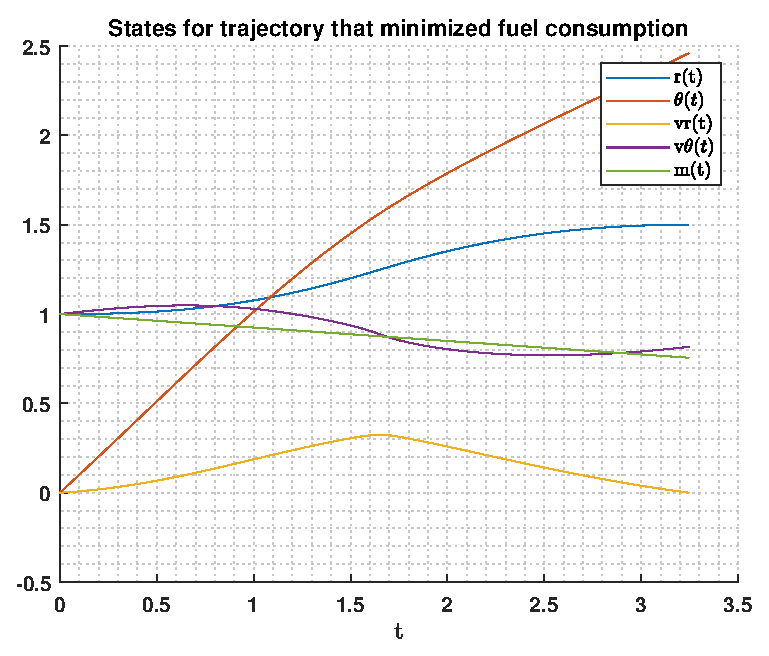
\includegraphics[scale=0.75]{indirectStates.eps}
    \caption{States for trajectory that minimizes fuel consumption}
	\label{fig:indirectStates}
\end{figure}
\begin{figure}
	\centering
	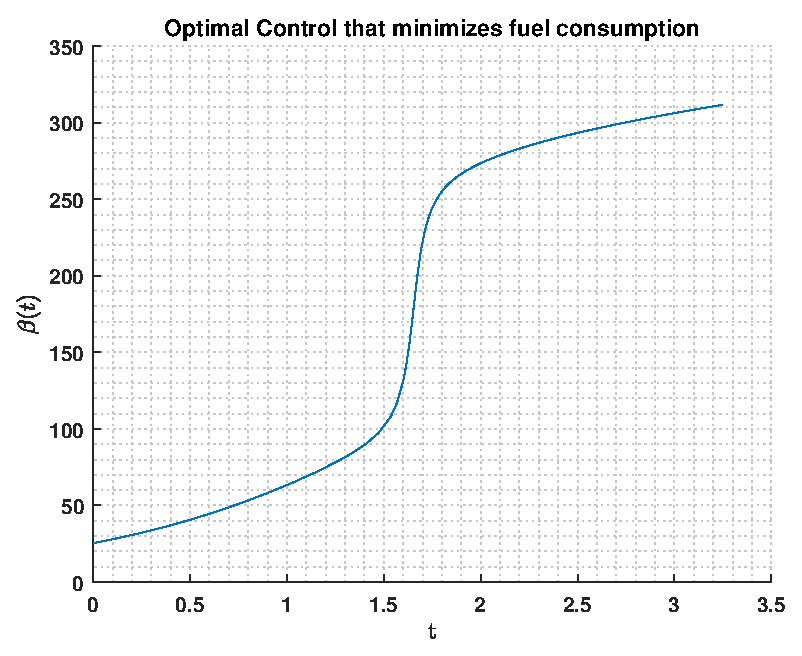
\includegraphics[scale=0.75]{indirectControl.eps}
	\caption{Optimal Control that minimizes fuel consumption}
	\label{fig:indirectControl}
\end{figure}
\FloatBarrier
\begin{table}
	\centering
	\begin{tabular}{||c c c c||} 
		\hline
		Iterations (s) & Sim Time & Terminal Time & Terminal Mass\\ [0.5ex] 
		\hline\hline
		27            & 0.321     &   3.247       & 0.755\\ [1ex]
		\hline
	\end{tabular}
\caption{Performance for Indirect Shooting}
\label{table:1}
\end{table}
\FloatBarrier
\subsubsection{Analysis of Indirect Shooting}
For this problem, the optimized terminal conditions were easily solvable using Indirect Shooting. The computation time was fast and the results were accurate. The only drawback to this methods is variational calculus must be used which is not always feasible and may, in some cases, increase computation. Also, for some problems, a single shoot might push the limits of CPU due to large time steps. 
\subsection{Indirect Multiple Shooting}
The second method used is Indirect Multiple Shooting, This method is much like Indirect Shooting but unlike integrating over a single time interval, multiple shooting allows you to break the single interval up into smaller sub-intervals. This is generally done to reduce the magnitude of numbers worked with during optimization. For Indirect Multiple Shooting, the intervals tested are: K = (2, 4, 8, 16).
\vspace{2mm}\newline
Figure \ref{fig:indirectMultiStates} shows the states for the trajectory that minimizes the fuel consumption for intervals \(K = 2\). Figure \ref{fig:indirectMultiControl} shows the optimal control to achieve the optimal trajectory for interval K = 2. The black asterisks in figures represent the start and end points of an interval. Much like Indirect Shooting, the optimized final time was found to be 3.247 while the terminal mass was 0.755. The solver converged after 16 iterations and an elapsed time of 0.4746 seconds.
\begin{figure}[hbt!]
	\centering
	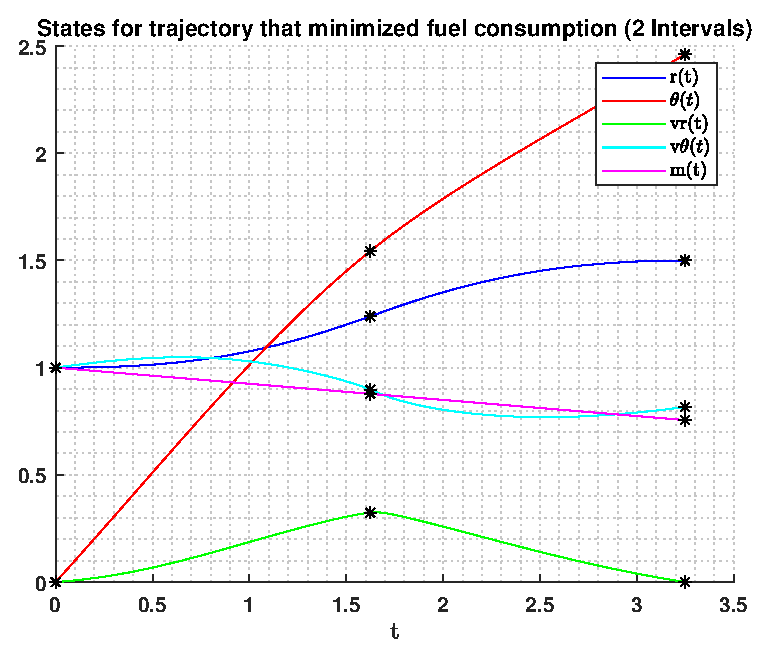
\includegraphics[scale=0.75]{indirectMultiStates.eps}
	\caption{States for trajectory that minimizes fuel consumption (2 intervals)}
	\label{fig:indirectMultiStates}
\end{figure}
\begin{figure}
	\centering
	\includegraphics[scale=0.75]{indirectMultiControl.eps}
	\caption{Optimal Control that minimizes fuel consumption (2 intervals)}
	\label{fig:indirectMultiControl}
\end{figure}
\FloatBarrier

Figure \ref{fig:indirectMultiStates4} shows the states for the trajectory that minimizes the fuel consumption for intervals \(K = 4\), while Figure \ref{fig:indirectMultiControl4} shows the optimal control to achieve this trajectory. The optimized terminal conditions are the same as those found with interval K = 2. The terminal time was \(t_f\) = 3.247 and the terminal mass was \(m\) = 0.755. For 4 intervals, the solver needed 14 iterations and an elapsed time of 1.067073 seconds.
\begin{figure}
	\centering
	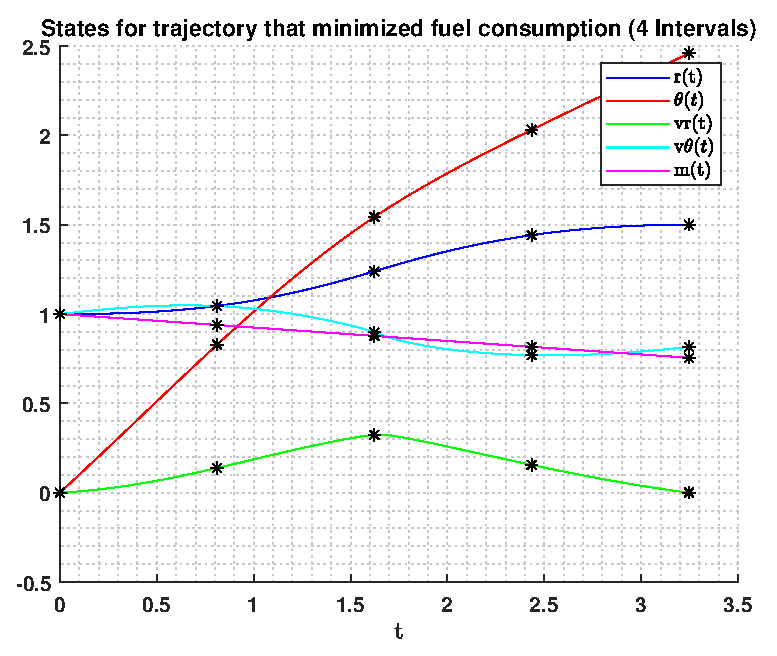
\includegraphics[scale=0.75]{indirectMultiStates4.eps}
	\caption{States for trajectory that minimizes fuel consumption (4 intervals)}
	\label{fig:indirectMultiStates4}
\end{figure}
\begin{figure}
	\centering
	\includegraphics[scale=0.75]{indirectMultiControl4.eps}
	\caption{Optimal Control that minimizes fuel consumption (4 intervals)}
	\label{fig:indirectMultiControl4}
\end{figure}
\FloatBarrier

Figure \ref{fig:indirectMultiStates8} shows the states for the trajectory that minimizes the fuel consumption for intervals \(K = 8\), while Figure \ref{fig:indirectMultiControl8} shows the optimal control to achieve this trajectory. The optimized terminal time and mass are 3.247 and 0.755, respectively. For 8 intervals, the solution converged after 18 iterations and an elapsed time of 3.368977 seconds. 
\begin{figure}
	\centering
	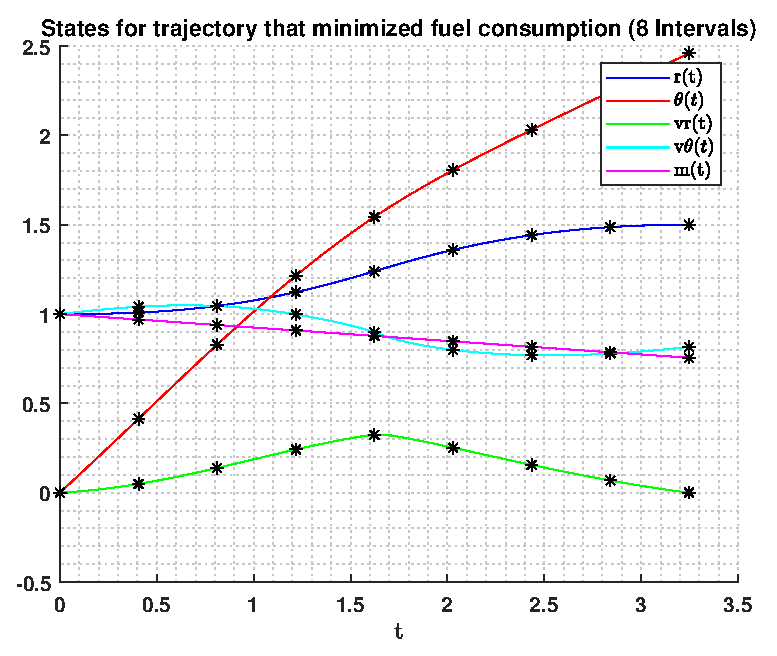
\includegraphics[scale=0.75]{indirectMultiStates8.eps}
	\caption{States for trajectory that minimizes fuel consumption (8 intervals)}
	\label{fig:indirectMultiStates8}
\end{figure}
\begin{figure}
	\centering
	\includegraphics[scale=0.75]{indirectMultiControl8.eps}
	\caption{Optimal Control that minimizes fuel consumption (8 intervals)}
	\label{fig:indirectMultiControl8}
\end{figure}
\FloatBarrier

The final Indirect Multiple Shooting case is with intervals K = 16. Figure \ref{fig:indirectMultiStates16} shows the states for the trajectory that minimizes the fuel consumption for intervals K = 16, while Figure \ref{fig:indirectMultiControl16} shows the optimal control to achieve this optimal trajectory. Just like all the other Indirect results, the terminal time and mass were optimized to be 3.247 and 0.755, respectively. However, for 16 interval the elapsed time increased to 12.280387 seconds. Lastly, the solution converged in 19 iterations.
tf = 3.25, mf = 0.755, 19 iterations, 16 intervals, Elapsed time is 12.280387 seconds.
\begin{figure}
	\centering
	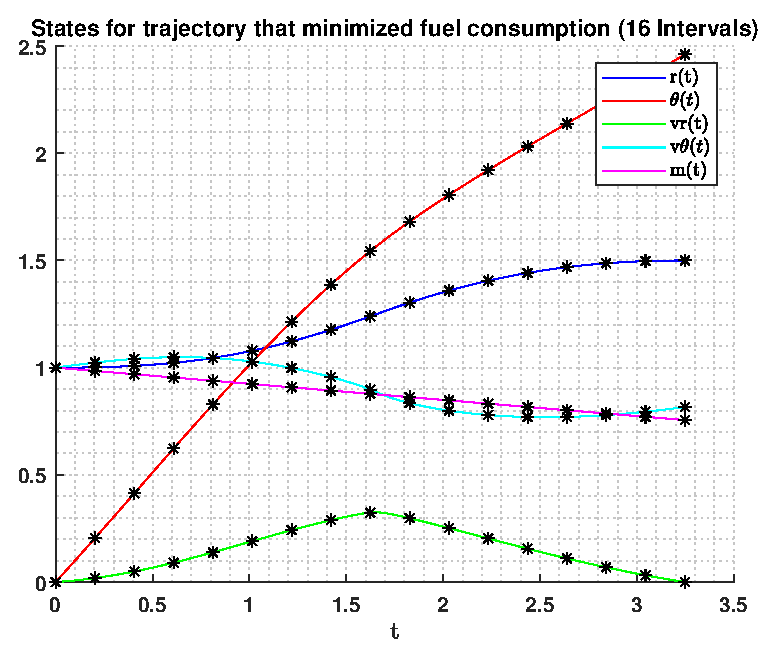
\includegraphics[scale=0.75]{indirectMultiStates16.eps}
	\caption{States for trajectory that minimizes fuel consumption (16 intervals)}
	\label{fig:indirectMultiStates16}
\end{figure}
\begin{figure}
	\centering
	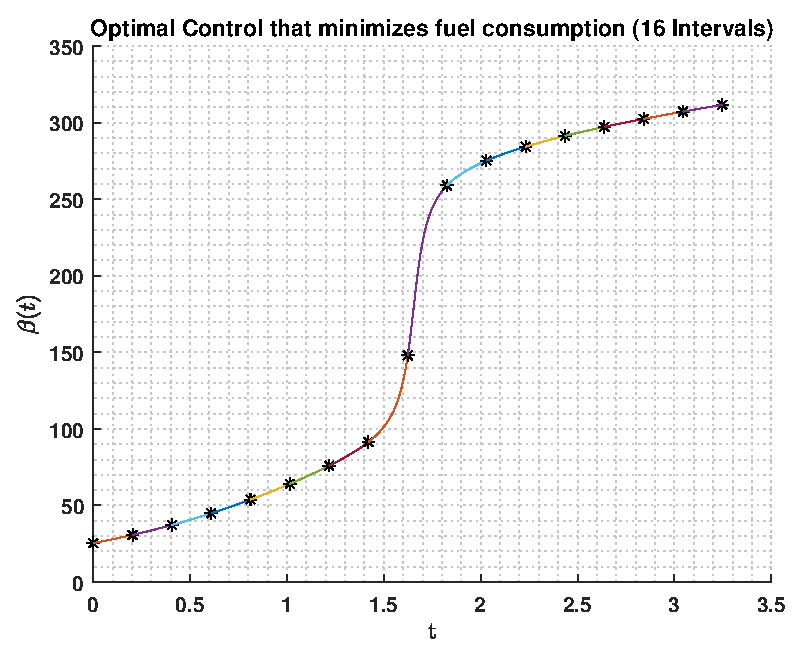
\includegraphics[scale=0.75]{indirectMultiControl16.eps}
	\caption{Optimal Control that minimizes fuel consumption (16 intervals)}
	\label{fig:indirectMultiControl16}
\end{figure}
\FloatBarrier
\begin{table}
    \centering
	\begin{tabular}{||c c c c c||} 
		\hline
		Intervals-K & Iterations (s) & Sim Time & Terminal Time & Terminal Mass\\ [0.5ex] 
		\hline\hline
		2           & 16            & 0.5110     &   3.24694      & 0.7555\\
		\hline
		4           & 19            & 0.9880     &   3.24694      & 0.7555\\ 
		\hline
		8           & 16            & 2.6119     &   3.24694      & 0.7555\\ 
		\hline
		16          & 19            & 10.9391    &  3.246944      & 0.7555\\ [1ex]
		\hline
	\end{tabular}
\caption{Performance for Indirect Multiple Shooting}
\label{table:2}
\end{table}
\FloatBarrier
\subsubsection{Analysis of Indirect Multiple Shooting}
Interestingly, all of the Indirect Multiple Shooting cases achieved the same optimized terminal conditions as the Indirect Shooting Method. This is most likely due to the fact that the errors at the interval points are minuscule and that the optimal control can be directly computed from the Hamiltonian. For each case, regardless of the number of intervals, the optimal control seems to be continuous. The main different between all the cases is that the computation time increases as you include more intervals. For this particular problem, Indirect Multiple Shooting does not show benefit over Indirect Shooting due to the terminal conditions being the same and higher computation costs.
\subsection{Direct Shooting}
The third numerical method used is Direct Shooting. This method is much different than the indirect methods in the sense that calculus of variations in not employed. Instead, when solving the differential equations, the control is parameterized by linear independent basis functions. For this study, the basis functions are polynomials with degree \(N\) ranging from 2 to 6. To get an optimized solution, the coefficients of the polynomials must be included in the optimization process. Also, as stated before, Direct Shooting was done on a \(\tau\) scale, rather than on a time scale. This is to be consistent with the next method, Direct Multiple Shooting.
\vspace{2mm}\newline 
The first Direct Shooting case is with the control being parameterized by a polynomial of degree \(N = 2\). Figure \ref{fig:directStatesPoly2} shows the states for the trajectory that minimizes the fuel consumption, while Figure \ref{fig:directControlPoly2} shows the optimal control to achieve this trajectory. Right away it is obvious that the results are much different from the previous Indirect Methods. This is because the control is approximated as a polynomial and it's obvious that from the Indirect Methods that the optimal control cant be well approximated with a single polynomial. For this case, single polynomial of degree \(N = 2\), the optimized terminal time and mass were found to be 3.866 and 0.708, respectively. The solution converged after 13 iterations and an elapsed time of 0.324692 seconds.
\begin{figure}
	\centering
	\includegraphics[scale=0.75]{directStatesPoly2.eps}
	\caption{States for trajectory that minimizes fuel consumption (\(N = 2\))}
	\label{fig:directStatesPoly2}
\end{figure}
\begin{figure}
	\centering
	\includegraphics[scale=0.75]{directControlPoly2.eps}
	\caption{Optimal Control that minimizes fuel consumption  (\(N = 2\))}
	\label{fig:directControlPoly2}
\end{figure}
\FloatBarrier

The second Direct Shooting case is with the control being parameterized by a polynomial of degree \(N = 3\). Figure \ref{fig:directStatesPoly3} shows the states for the trajectory that minimizes the fuel consumption, while Figure \ref{fig:directControlPoly3} shows the optimal control to achieve this trajectory. Again, it is obvious that the single polynomial does not represent the optimal control showed with the indirect methods. For this case, the optimized terminal time and mass were found to be 3.511 and 0.735, respectively. The solution converged after 23 iterations and an elapsed time of 0.458609 seconds.
\begin{figure}
	\centering
	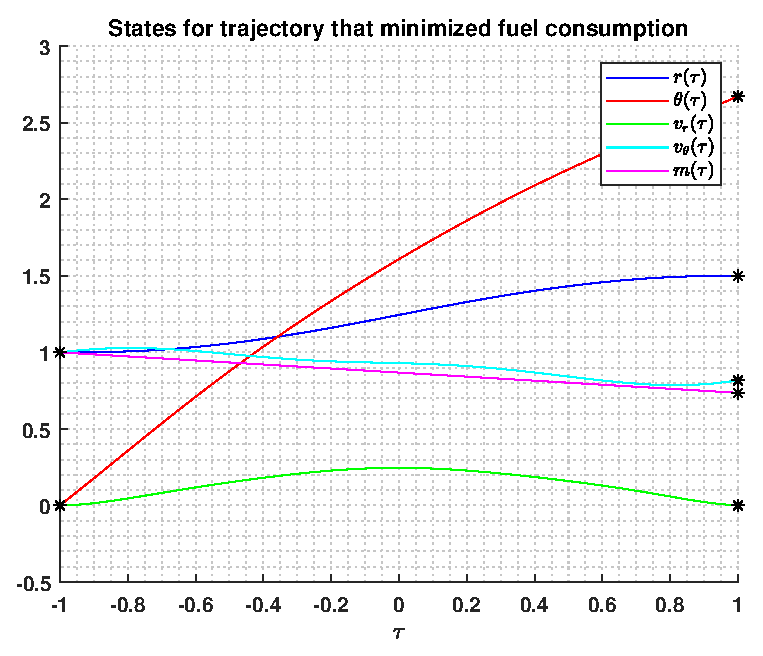
\includegraphics[scale=0.75]{directStatesPoly3.eps}
	\caption{States for trajectory that minimizes fuel consumption (\(N = 3\))}
	\label{fig:directStatesPoly3}
\end{figure}
\begin{figure}
	\centering
	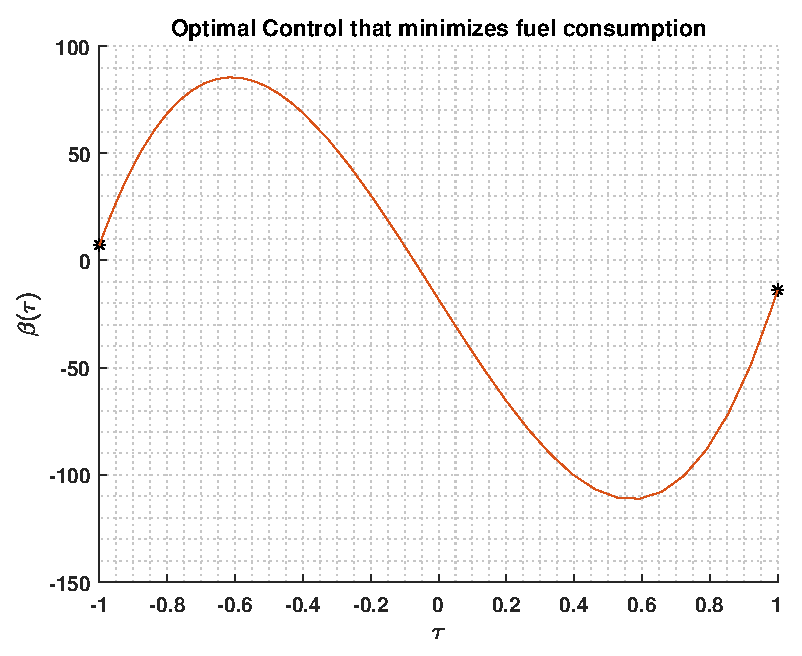
\includegraphics[scale=0.75]{directControlPoly3.eps}
	\caption{Optimal Control that minimizes fuel consumption (\(N = 3\))}
	\label{fig:directControlPoly3}
\end{figure}
\FloatBarrier

The next Direct Shooting case is with the control being parameterized by a polynomial of degree \(N = 4\). Figure \ref{fig:directStatesPoly4} shows the states for the trajectory that minimizes the fuel consumption, while Figure \ref{fig:directControlPoly4} shows the optimal control to achieve this trajectory. For this case, the optimized terminal time and mass were found to be 3.472 and 0.73855, respectively. The solution converged after 26 iterations and an elapsed time of 0.617611 seconds.
\begin{figure}
	\centering
	\includegraphics[scale=0.75]{directStatesPoly4.eps}
	\caption{States for trajectory that minimizes fuel consumption (\(N = 4\))}
	\label{fig:directStatesPoly4}
\end{figure}
\begin{figure}
	\centering
	\includegraphics[scale=0.75]{directControlPoly4.eps}
	\caption{Optimal Control that minimizes fuel consumption (\(N = 4\))}
	\label{fig:directControlPoly4}
\end{figure}
\FloatBarrier

The fourth Direct Shooting case is with the control being parameterized by a polynomial of degree \(N = 5\). Figure \ref{fig:directStatesPoly5} shows the states for the trajectory that minimizes the fuel consumption, while Figure \ref{fig:directControlPoly5} shows the optimal control to achieve this trajectory. For this case, the optimized terminal time and mass were found to be 3.364 and 0.7466, respectively. The solution converged after 41 iterations and an elapsed time of 0.826949 seconds.
\begin{figure}
	\centering
	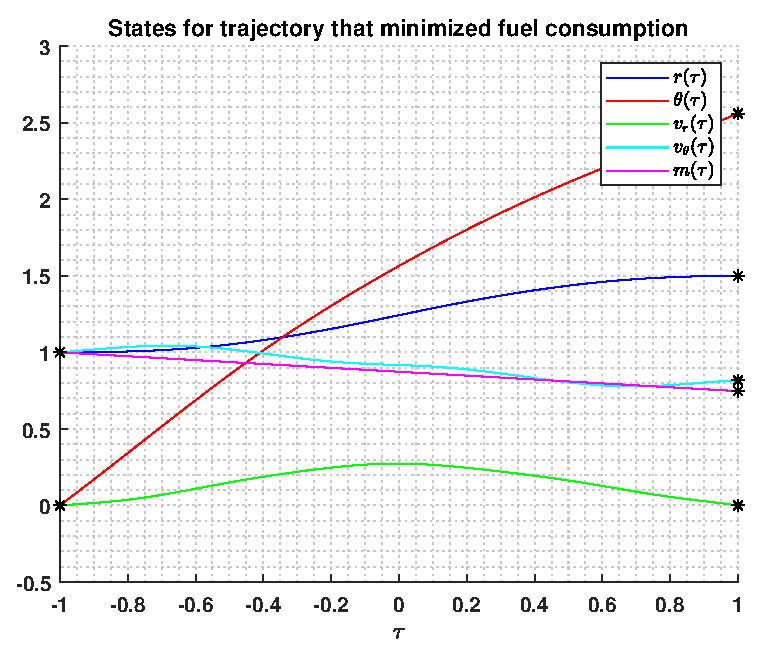
\includegraphics[scale=0.75]{directStatesPoly5.eps}
	\caption{States for trajectory that minimizes fuel consumption (\(N = 5\))}
	\label{fig:directStatesPoly5}
\end{figure}
\begin{figure}
	\centering
	\includegraphics[scale=0.75]{directControlPoly5.eps}
	\caption{Optimal Control that minimizes fuel consumption (\(N = 5\))}
	\label{fig:directControlPoly5}
\end{figure}
\FloatBarrier

The final Direct Shooting case is with the control being parameterized by a polynomial of degree \(N = 6\). Figure \ref{fig:directStatesPoly6} shows the states for the trajectory that minimizes the fuel consumption, while Figure \ref{fig:directControlPoly6} shows the optimal control to achieve this trajectory. For this case, the optimized terminal time and mass were found to be 3.361 and 0.74696, respectively. The solution converged after 41 iterations and an elapsed time of 1.017488 seconds.
\begin{figure}
	\centering
	\includegraphics[scale=0.75]{directStatesPoly6.eps}
	\caption{States for trajectory that minimizes fuel consumption (\(N = 6\))}
	\label{fig:directStatesPoly6}
\end{figure}
\begin{figure}
	\centering
	\includegraphics[scale=0.75]{directControlPoly6.eps}
	\caption{Optimal Control that minimizes fuel consumption (\(N = 6\))}
	\label{fig:directControlPoly6}
\end{figure}
\FloatBarrier
\begin{table}
	\centering
	\begin{tabular}{||c c c c c||} 
		\hline
		Degree-N & Iterations (s) & Sim Time & Terminal Time & Terminal Mass\\ [0.5ex] 
		\hline\hline
		2           & 13            & 0.3289     &  3.8662     & 0.7555\\
		\hline
		3           & 23            & 0.2474     &  3.5109     & 0.7089\\ 
		\hline
		4           & 26            & 0.3590     &  3.4723     & 0.7356\\ 
		\hline
		5           & 41            & 0.4678     &  3.3641     & 0.7467\\ 
		\hline
		6           & 51            & 0.6769     &  3.3611     & 0.7469\\ [1ex]
		\hline
	\end{tabular}
	\caption{Performance for Direct Shooting}
	\label{table:3}
\end{table}
\FloatBarrier
\subsubsection{Analysis of Direct Shooting}
The Direct Shooting numerical method produced much different results than that of the two indirect methods. It is evident that the control being parameterized as a single polynomial basis function does not produce as optimized results as employing the calculus of variations. However, there are some highlights to the Direct Shooting method which are that it is much simpler to employ. Also, for single Direct Shooting case, the computation time is very efficient. The case with polynomial degree \(N = 6\) was the most computationally heavy and only took 1.017488 to converge on a solution. While Indirect Shooting only took 0.321 seconds, Indirect Multiple Shooting ranged from 0.4746 to 12.28 seconds. Out of these methods the preferred method really comes down to the requirements. The largest terminal mass for the Direct Shooting method was 0.747 when the control is parameterized with a polynomial of degree \(N = 6\). Depending on the scale, this could be a massive difference from the optimized terminal mass using the indirect methods. This results in an approximately 1\% difference in mass.

\subsection{Direct Multiple Shooting}
The final numerical method used to solve the optimal control problem is Direct Multiple Shooting. Direct Multiple Shooting similar to Direct Shooting but utilized \(K\) intervals like Indirect Multiple Shooting. Direct Multiple Shooting allows for different sets of polynomial coefficients for each interval. For this study, Direct Multiple Shooting was performed for intervals \(K = (2,4,8,16)\) and with the control parameterized with polynomial of degree \(N = (2,3,4,5,6)\).
\vspace{2mm}\newline 
The first set of Direct Multiple Shooting cases are performed with the degree polynomial \(N = 2\) and intervals \(K = (2,4,8,16)\). Figure \ref{fig:directStatesK2Poly2} shows the states for the trajectory that minimizes the fuel consumption for \(K = 2\) and  \(N = 2\), while Figure \ref{fig:directControlK2Poly2} shows the optimal control to achieve this trajectory. It is instantly noticeable that the optimal control is much closer to that of the indirect methods than any of the Direct Shooting cases. This is because having two intervals allows for the control to be parameterized with two different polynomials rather than one. For this case, the terminal time and mass were found to be 3.2489 and 0.755, respectively. The solution converged after 33 iterations and an elapsed time of 0.937331 seconds.
\begin{figure}
	\centering
	\includegraphics[scale=0.75]{directStatesK2Poly2.eps}
	\caption{States for trajectory that minimizes fuel consumption (\(K:2\ , N:2\))}
	\label{fig:directStatesK2Poly2}
\end{figure}
\begin{figure}
	\centering
	\includegraphics[scale=0.75]{directControlK2Poly2.eps}
	\caption{Optimal Control that minimizes fuel consumption (\(K:2\ , N:2\))}
	\label{fig:directControlK2Poly2}
\end{figure}
\FloatBarrier

Figure \ref{fig:directStatesK4Poly2} shows the states for the trajectory that minimizes the fuel consumption for \(K = 4\) and  \(N = 2\), while Figure \ref{fig:directControlK4Poly2} shows the optimal control to achieve this trajectory. For this case, the optimized terminal time and mass converged at 3.248 and  0.755, respectively. The solution converged after 64 iterations and an elapsed time of 3.975852 seconds. Already, it is noticeable that the optimized terminal conditions are very similar to those using the indirect methods. While the optimized conditions are similar, the computational cost are a little higher.
\begin{figure}
	\centering
	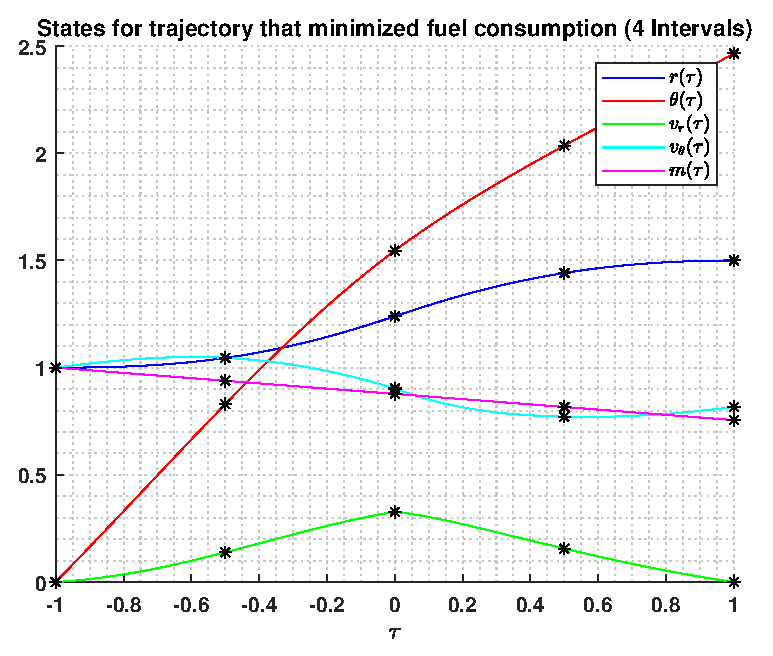
\includegraphics[scale=0.75]{directStatesK4Poly2.eps}
	\caption{States for trajectory that minimizes fuel consumption (\(K:4\ , N:2\))}
	\label{fig:directStatesK4Poly2}
\end{figure}
\begin{figure}
	\centering
	\includegraphics[scale=0.75]{directControlK4Poly2.eps}
	\caption{Optimal Control that minimizes fuel consumption (\(K:4\ , N:2\))}
	\label{fig:directControlK4Poly2}
\end{figure}
\FloatBarrier

Figure \ref{fig:directStatesK8Poly2} shows the states for the trajectory that minimizes the fuel consumption for \(K = 8\) and  \(N = 2\), while Figure \ref{fig:directControlK8Poly2} shows the optimal control to achieve this trajectory. Similar to two intervals, four intervals allows for an optimized terminal time and mass of 3.248 and 0.755, respectively. However, with four intervals, the solution converged after 94 iterations and an elapsed time of 18.411803 seconds. By this point, the addition of more intervals does not produce a more optimized solution while the computation cost continues to get larger.

\begin{figure}
	\centering
	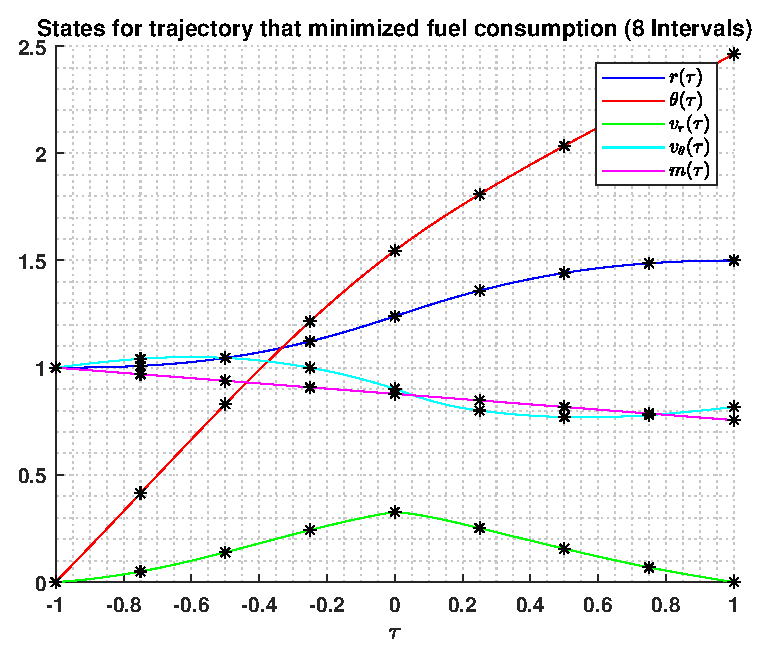
\includegraphics[scale=0.75]{directStatesK8Poly2.eps}
	\caption{States for trajectory that minimizes fuel consumption (\(K:8\ , N:2\))}
	\label{fig:directStatesK8Poly2}
\end{figure}
\begin{figure}
	\centering
	\includegraphics[scale=0.75]{directControlK8Poly2.eps}
	\caption{Optimal Control that minimizes fuel consumption (\(K:8\ , N:2\))}
	\label{fig:directControlK8Poly2}
\end{figure}
\FloatBarrier

Figure \ref{fig:directStatesK16Poly2} shows the states for the trajectory that minimizes the fuel consumption for \(K = 16\) and  \(N = 2\), while Figure \ref{fig:directControlK16Poly2} shows the optimal control to achieve this trajectory. The terminal time and mass were optimized to be 3.248 and 0.755, respectively. The solution converged after 112 iterations and an elapsed time of 80.721927 seconds. Interestingly about this case, a solution was originally computed with lower coefficient bounds which prevented the terminal conditions from being as optimal as previous cases. Once the bounds were opened, similar optimized terminal conditions were achieved.
\begin{figure}
	\centering
	\includegraphics[scale=0.75]{directStatesK16Poly2.eps}
	\caption{States for trajectory that minimizes fuel consumption (\(K:16\ , N:2\))}
	\label{fig:directStatesK16Poly2}
\end{figure}
\begin{figure}
	\centering
	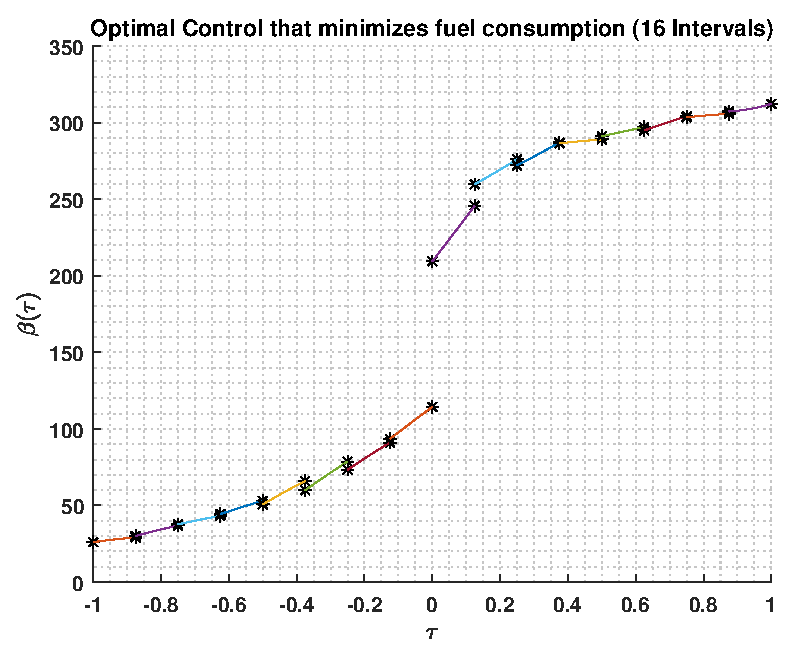
\includegraphics[scale=0.75]{directControlK16Poly2.eps}
	\caption{Optimal Control that minimizes fuel consumption (\(K:16\ , N:2\))}
	\label{fig:directControlK16Poly2}
\end{figure}
\FloatBarrier

The next set of Direct Multiple Shooting cases are performed with the degree polynomial \(N = 3\) and intervals \(K = (2,4,8,16)\). Figure \ref{fig:directStatesK2Poly3} shows the states for the trajectory that minimizes the fuel consumption for \(K = 2\) and  \(N = 3\), while Figure \ref{fig:directControlK2Poly3} shows the optimal control to achieve this trajectory. The results for this case are similar to the previous Direct Multiple Shooting results. The terminal time was optimized to be 3.248 while the terminal mass was optimized to be 0.755. The solution for this case converged after 46 iterations and an elapsed time of 1.24360 seconds.
\begin{figure}
	\centering
	\includegraphics[scale=0.75]{directStatesK2Poly3.eps}
	\caption{States for trajectory that minimizes fuel consumption (\(K:2\ , N:3\))}
	\label{fig:directStatesK2Poly3}
\end{figure}
\begin{figure}
	\centering
	\includegraphics[scale=0.75]{directControlK2Poly3.eps}
	\caption{Optimal Control that minimizes fuel consumption (\(K:2\ , N:3\))}
	\label{fig:directControlK2Poly3}
\end{figure}
\FloatBarrier

Figure \ref{fig:directStatesK4Poly3} shows the states for the trajectory that minimizes the fuel consumption for \(K = 4\) and  \(N = 3\), while Figure \ref{fig:directControlK4Poly3} shows the optimal control to achieve this trajectory. The optimized terminal time and mass are 3.248 and 0.7554, respectively. The solution converged after 69 iterations and an elapsed time of 4.702343 seconds.
\begin{figure}
	\centering
	\includegraphics[scale=0.75]{directStatesK4Poly3.eps}
	\caption{States for trajectory that minimizes fuel consumption (\(K:4\ , N:3\))}
	\label{fig:directStatesK4Poly3}
\end{figure}
\begin{figure}
	\centering
	\includegraphics[scale=0.75]{directControlK4Poly3.eps}
	\caption{Optimal Control that minimizes fuel consumption (\(K:4\ , N:3\))}
	\label{fig:directControlK4Poly3}
\end{figure}
\FloatBarrier

Figure \ref{fig:directStatesK8Poly3} shows the states for the trajectory that minimizes the fuel consumption for \(K = 8\) and  \(N = 3\), while Figure \ref{fig:directControlK8Poly3} shows the optimal control to achieve this trajectory. The optimized terminal time and mass are 3.248 and 0.7554, respectively. The solution converged after 93 iterations and an elapsed time of 20.779223 seconds. Similar to Direct Multiple Shooting with polynomial degree \(N = 2\), increase in intervals, does not improve the optimized solution and continues to increase in computation cost.
\begin{figure}
	\centering
	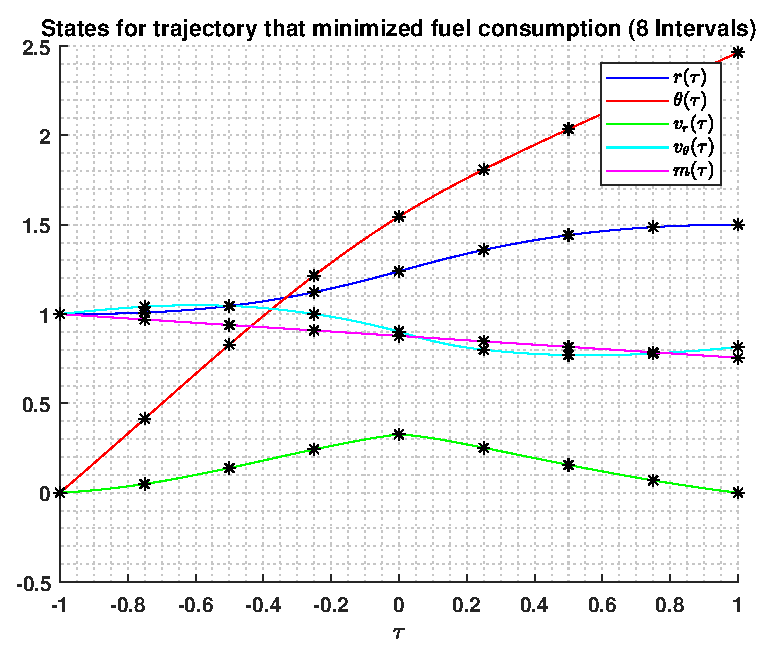
\includegraphics[scale=0.75]{directStatesK8Poly3.eps}
	\caption{States for trajectory that minimizes fuel consumption (\(K:8\ , N:3\))}
	\label{fig:directStatesK8Poly3}
\end{figure}
\begin{figure}
	\centering
	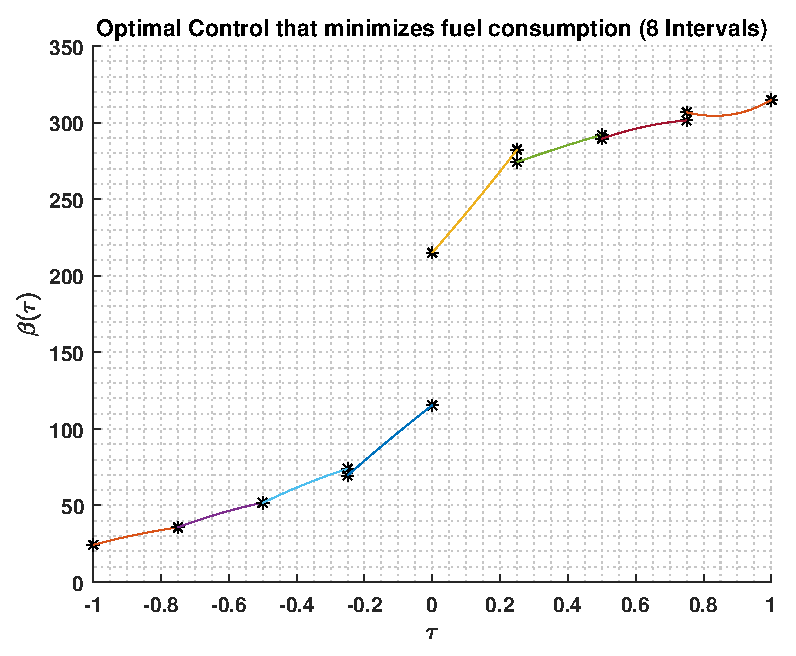
\includegraphics[scale=0.75]{directControlK8Poly3.eps}
	\caption{Optimal Control that minimizes fuel consumption (\(K:8\ , N:3\))}
	\label{fig:directControlK8Poly3}
\end{figure}
\FloatBarrier

The last case where the control is parameterized by a \(3^{rd}\) degree polynomial is with intervals \(K = 16\). Figure \ref{fig:directStatesK16Poly3} shows the states for the trajectory that minimizes the fuel consumption, while Figure \ref{fig:directControlK16Poly3} shows the optimal control to achieve this trajectory. The optimized terminal time and mass are 3.248 and 0.7554, respectively. The solution converged after 128 iterations and an elapsed time of 105.069901 seconds. Just like 16 interval case with \(2^{nd}\) degree polynomial control, the solution was further optimized when the polynomial coefficient bounds were opened. Increasing the bounds not only allowed for a more optimized solution, but also improved the computation cost.
\begin{figure}
	\centering
	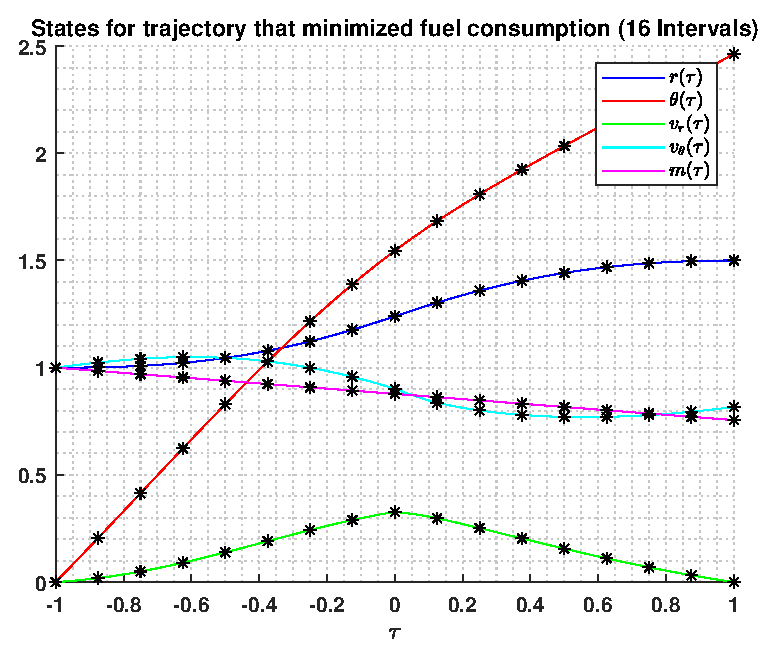
\includegraphics[scale=0.75]{directStatesK16Poly3.eps}
	\caption{States for trajectory that minimizes fuel consumption (\(K:16\ , N:3\))}
	\label{fig:directStatesK16Poly3}
\end{figure}
\begin{figure}
	\centering
	\includegraphics[scale=0.75]{directControlK16Poly3.eps}
	\caption{Optimal Control that minimizes fuel consumption (\(K:16\ , N:3\))}
	\label{fig:directControlK16Poly3}
\end{figure}
\FloatBarrier

The third set of Direct Multiple Shooting cases are performed with the control parameterized by a \(4^{th}\) degree polynomial for intervals \(K = (2,4,8,16)\). Figure \ref{fig:directStatesK2Poly4} shows the states for the trajectory that minimizes the fuel consumption for \(K = 2\) and  \(N = 4\), while Figure \ref{fig:directControlK2Poly4} shows the optimal control to achieve this trajectory. The optimal control looks similar to that of the other direct multiple shooting two-interval cases. The optimized terminal time and mass are 3.248 and 0.7553, respectively. The optimal solution converged after 41 iterations and an elapsed time of 1.313428 seconds. Comparing with the other direct multiple shooting two-interval interval cases, it seems that the computation cost increases as the polynomial degree gets larger. This makes sense because an extra degree requires extra optimization.
\begin{figure}
	\centering
	\includegraphics[scale=0.75]{directStatesK2Poly4.eps}
	\caption{States for trajectory that minimizes fuel consumption (\(K:2\ , N:4\))}
	\label{fig:directStatesK2Poly4}
\end{figure}
\begin{figure}
	\centering
	\includegraphics[scale=0.75]{directControlK2Poly4.eps}
	\caption{Optimal Control that minimizes fuel consumption (\(K:2\ , N:4\))}
	\label{fig:directControlK2Poly4}
\end{figure}
\FloatBarrier

Figure \ref{fig:directStatesK4Poly4} shows the states for the trajectory that minimizes the fuel consumption for \(K = 4\) and  \(N = 4\), while Figure \ref{fig:directControlK4Poly4} shows the optimal control to achieve this trajectory. The optimized terminal time and mass are 3.2479 and 0.7554, respectively. The optimal solution converged after 65 iterations and an elapsed time of 4.854514 seconds.
\begin{figure}
	\centering
	\includegraphics[scale=0.75]{directStatesK4Poly4.eps}
	\caption{States for trajectory that minimizes fuel consumption (\(K:4\ , N:4\))}
	\label{fig:directStatesK4Poly4}
\end{figure}
\begin{figure}
	\centering
	\includegraphics[scale=0.75]{directControlK4Poly4.eps}
	\caption{Optimal Control that minimizes fuel consumption (\(K:4\ , N:4\))}
	\label{fig:directControlK4Poly4}
\end{figure}
\FloatBarrier

Figure \ref{fig:directStatesK8Poly4} shows the states for the trajectory that minimizes the fuel consumption for \(K = 8\) and  \(N = 4\), while Figure \ref{fig:directControlK8Poly4} shows the optimal control to achieve this trajectory. The optimized terminal time and mass are 3.2481 and 0.7554, respectively. The optimal solution converged after 90 iterations and an elapsed time of 22.244379 seconds.
\begin{figure}
	\centering
	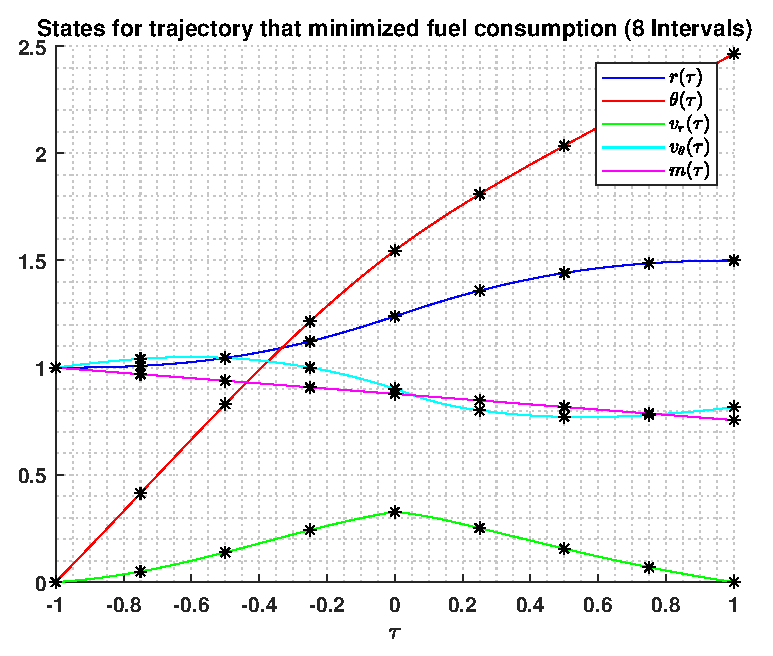
\includegraphics[scale=0.75]{directStatesK8Poly4.eps}
	\caption{States for trajectory that minimizes fuel consumption (\(K:8\ , N:4\))}
	\label{fig:directStatesK8Poly4}
\end{figure}
\begin{figure}
	\centering
	\includegraphics[scale=0.75]{directControlK8Poly4.eps}
	\caption{Optimal Control that minimizes fuel consumption (\(K:8\ , N:4\))}
	\label{fig:directControlK8Poly4}
\end{figure}
\FloatBarrier

Figure \ref{fig:directStatesK16Poly4} shows the states for the trajectory that minimizes the fuel consumption for \(K = 16\) and  \(N = 4\), while Figure \ref{fig:directControlK16Poly4} shows the optimal control to achieve this trajectory. The optimized terminal time and mass are 3.2481 and 0.7554, respectively. The optimal solution converged after 142 iterations and an elapsed time of 129.659140 seconds. Again, like the other 16-interval cases, the polynomial coefficient bounds were opened for better optimization. 
\begin{figure}
	\centering
	\includegraphics[scale=0.75]{directStatesK16Poly4.eps}
	\caption{States for trajectory that minimizes fuel consumption (\(K:16\ , N:4\))}
	\label{fig:directStatesK16Poly4}
\end{figure}
\begin{figure}
	\centering
	\includegraphics[scale=0.75]{directControlK16Poly4.eps}
	\caption{Optimal Control that minimizes fuel consumption (\(K:16\ , N:4\))}
	\label{fig:directControlK16Poly4}
\end{figure}
\FloatBarrier

The next set of Direct Multiple Shooting cases are the control parameterized by a \(5^{th}\) degree polynomial for intervals \(K = (2,4,8,16)\). Figure \ref{fig:directStatesK2Poly5} shows the states for the trajectory that minimizes the fuel consumption for \(K = 2\) and  \(N = 5\), while Figure \ref{fig:directControlK2Poly5} shows the optimal control to achieve this trajectory. The optimized terminal time and mass are 3.2485 and 0.7553, respectively. The optimal solution converged after 37 iterations and an elapsed time of 1.345495 seconds. Regardless of the polynomial degree, the optimized control seems to look very similar for each interval.
\begin{figure}
	\centering
	\includegraphics[scale=0.75]{directStatesK2Poly5.eps}
	\caption{States for trajectory that minimizes fuel consumption (\(K:2\ , N:5\))}
	\label{fig:directStatesK2Poly5}
\end{figure}
\begin{figure}
	\centering
	\includegraphics[scale=0.75]{directControlK2Poly5.eps}
	\caption{Optimal Control that minimizes fuel consumption (\(K:2\ , N:5\))}
	\label{fig:directControlK2Poly5}
\end{figure}
\FloatBarrier

Figure \ref{fig:directStatesK4Poly5} shows the states for the trajectory that minimizes the fuel consumption for \(K = 4\) and  \(N = 5\), while Figure \ref{fig:directControlK4Poly5} shows the optimal control to achieve this trajectory. The optimized terminal time and mass are 3.2479 and 0.7554, respectively. The optimal solution converged after 67 iterations and an elapsed time of 5.625521 seconds.
\begin{figure}
	\centering
	\includegraphics[scale=0.75]{directStatesK4Poly5.eps}
	\caption{States for trajectory that minimizes fuel consumption (\(K:4\ , N:5\))}
	\label{fig:directStatesK4Poly5}
\end{figure}
\begin{figure}
	\centering
	\includegraphics[scale=0.75]{directControlK4Poly5.eps}
	\caption{Optimal Control that minimizes fuel consumption (\(K:4\ , N:5\))}
	\label{fig:directControlK4Poly5}
\end{figure}
\FloatBarrier

Figure \ref{fig:directStatesK8Poly5} shows the states for the trajectory that minimizes the fuel consumption for \(K = 8\) and  \(N = 5\), while Figure \ref{fig:directControlK8Poly5} shows the optimal control to achieve this trajectory. The optimized terminal time and mass are 3.248 and 0.7554, respectively. The optimal solution converged after 98 iterations and an elapsed time of 27.079276 seconds.
\begin{figure}
	\centering
	\includegraphics[scale=0.75]{directStatesK8Poly5.eps}
	\caption{States for trajectory that minimizes fuel consumption (\(K:8\ , N:5\))}
	\label{fig:directStatesK8Poly5}
\end{figure}
\begin{figure}
	\centering
	\includegraphics[scale=0.75]{directControlK8Poly5.eps}
	\caption{Optimal Control that minimizes fuel consumption (\(K:8\ , N:5\))}
	\label{fig:directControlK8Poly5}
\end{figure}
\FloatBarrier

Figure \ref{fig:directStatesK16Poly5} shows the states for the trajectory that minimizes the fuel consumption for \(K = 16\) and  \(N = 5\), while Figure \ref{fig:directControlK16Poly5} shows the optimal control to achieve this trajectory. The optimized terminal time and mass are 3.248 and 0.7554, respectively. The optimal solution converged after 136 iterations and an elapsed time of 138.476447 seconds. Again, like the other 16-interval cases, the polynomial coefficient bounds were opened for better optimization. The terminal time changed from 3.25 to 3.248 which is a 0.06\% difference. 
\begin{figure}
	\centering
	\includegraphics[scale=0.75]{directStatesK16Poly5.eps}
	\caption{States for trajectory that minimizes fuel consumption (\(K:16\ , N:5\))}
	\label{fig:directStatesK16Poly5}
\end{figure}
\begin{figure}
	\centering
	\includegraphics[scale=0.75]{directControlK16Poly5.eps}
	\caption{Optimal Control that minimizes fuel consumption (\(K:16\ , N:5\))}
	\label{fig:directControlK16Poly5}
\end{figure}
\FloatBarrier

The last set of Direct Multiple Shooting cases are those with the control parameterized by a \(6^{th}\) degree polynomial for intervals \(K = (2,4,8,16)\). Figure \ref{fig:directStatesK2Poly6} shows the states for the trajectory that minimizes the fuel consumption for \(K = 2\) and  \(N = 6\), while Figure \ref{fig:directControlK2Poly6} shows the optimal control to achieve this trajectory. The optimized terminal time and mass are 3.2486 and 0.7554, respectively. The optimal solution converged after 48 iterations and an elapsed time of 1.721967 seconds.
\begin{figure}
	\centering
	\includegraphics[scale=0.75]{directStatesK2Poly6.eps}
	\caption{States for trajectory that minimizes fuel consumption (\(K:2\ , N:6\))}
	\label{fig:directStatesK2Poly6}
\end{figure}
\begin{figure}
	\centering
	\includegraphics[scale=0.75]{directControlK2Poly6.eps}
	\caption{Optimal Control that minimizes fuel consumption (\(K:2\ , N:6\))}
	\label{fig:directControlK2Poly6}
\end{figure}
\FloatBarrier

Figure \ref{fig:directStatesK4Poly6} shows the states for the trajectory that minimizes the fuel consumption for \(K = 4\) and  \(N = 6\), while Figure \ref{fig:directControlK4Poly6} shows the optimal control to achieve this trajectory. The optimized terminal time and mass are 3.2479 and 0.755, respectively. The optimal solution converged after 63 iterations and an elapsed time of 5.7287548 seconds.
\begin{figure}
	\centering
	\includegraphics[scale=0.75]{directStatesK4Poly6.eps}
	\caption{States for trajectory that minimizes fuel consumption (\(K:4\ , N:6\))}
	\label{fig:directStatesK4Poly6}
\end{figure}
\begin{figure}
	\centering
	\includegraphics[scale=0.75]{directControlK4Poly6.eps}
	\caption{Optimal Control that minimizes fuel consumption (\(K:4\ , N:6\))}
	\label{fig:directControlK4Poly6}
\end{figure}
\FloatBarrier

Figure \ref{fig:directStatesK8Poly6} shows the states for the trajectory that minimizes the fuel consumption for \(K = 8\) and  \(N = 6\), while Figure \ref{fig:directControlK8Poly6} shows the optimal control to achieve this trajectory. The optimized terminal time and mass are 3.248 and 0.7554, respectively. The optimal solution converged after 107 iterations and an elapsed time of 31.923118 seconds. 
\begin{figure}
	\centering
	\includegraphics[scale=0.75]{directStatesK8Poly6.eps}
	\caption{States for trajectory that minimizes fuel consumption (\(K:8\ , N:6\))}
	\label{fig:directStatesK8Poly6}
\end{figure}
\begin{figure}
	\centering
	\includegraphics[scale=0.75]{directControlK8Poly6.eps}
	\caption{Optimal Control that minimizes fuel consumption (\(K:8\ , N:6\))}
	\label{fig:directControlK8Poly6}
\end{figure}
\FloatBarrier

The last case where the control is parameterized by a \(6^{th}\) degree polynomial is with intervals \(K = 16\). Figure \ref{fig:directStatesK16Poly6} shows the states for the trajectory that minimizes the fuel consumption, while Figure \ref{fig:directControlK16Poly6} shows the optimal control to achieve this trajectory. The optimized terminal time and mass are 3.248 and 0.7554, respectively. The solution converged after 128 iterations and an elapsed time of  184.219058 seconds. Just like 16 interval cases with \(N\) degree polynomial control, the solution was further optimized when the polynomial coefficient bounds were opened. Increasing the bounds not only allowed for a more optimized solution, but also improved the computation cost. 
\begin{figure}
	\centering
	\includegraphics[scale=0.75]{directStatesK16Poly6.eps}
	\caption{States for trajectory that minimizes fuel consumption (\(K:16\ , N:6\))}
	\label{fig:directStatesK16Poly6}
\end{figure}
\begin{figure}
	\centering
	\includegraphics[scale=0.75]{directControlK16Poly6.eps}
	\caption{Optimal Control that minimizes fuel consumption (\(K:16\ , N:6\))}
	\label{fig:directControlK16Poly6}
\end{figure}
\FloatBarrier
\begin{table}
	\centering
	\begin{tabular}{||c c c c c c||} 
		\hline
		Degree-N & Intervals-K & Iterations (s) & Sim Time & Terminal Time & Terminal Mass\\ [0.5ex] 
		\hline\hline
		2        & 2           & 33             & 0.7972   & 3.2489     & 0.7554\\ 
		\hline
		2        & 4           & 59             & 3.0869   & 3.2479     & 0.7554\\
		\hline
		2        & 8           & 75             & 13.8941  & 3.2478     & 0.7554\\
		\hline
		2        & 16          & 112            & 79.1192  & 3.2477     & 0.7554\\
		\hline
		3        & 2           & 45             & 0.8537   & 3.2480     & 0.7554\\
		\hline
		3        & 4           & 63             & 3.5958   & 3.2479     & 0.7554\\
		\hline
		3        & 8           & 92             & 19.576   & 3.2478     & 0.7554\\
		\hline
		3        & 16          & 128            & 101.136  & 3.2477     & 0.7554\\
		\hline
		4        & 2           & 38             & 0.7176   & 3.2483     & 0.7554\\
		\hline
		4        & 4           & 66             & 4.1511   & 3.2479     & 0.7554\\
		\hline
		4        & 8           & 87             & 20.2003  & 3.2479     & 0.7554\\
		\hline
		4        & 16          & 142            & 124.693  & 3.2475     & 0.7555\\
		\hline
		5        & 2           & 38             & 0.8166   & 3.2485     & 0.7554\\
		\hline
		5        & 4           & 65             & 4.7263   & 3.2480     & 0.7554\\
		\hline
		5        & 8           & 94             & 24.1589  & 3.2478     & 0.7554\\
		\hline
		5        & 16          & 136            & 132.165  & 3.2476     & 0.7555\\
		\hline
		6        & 2           & 47             & 1.1136   & 3.2486     & 0.7555\\
		\hline
		6        & 4           & 64             & 4.9823   & 3.2480     & 0.7554\\
		\hline
		6        & 8           & 117            & 35.1663  & 3.2478     & 0.7554\\
		\hline
		6        & 16          & 145            & 153.775  & 3.2476     & 0.7555\\ [1ex]
		\hline
	\end{tabular}
	\caption{Performance for Direct Multiple Shooting}
	\label{table:4}
\end{table}
\begin{figure}
	\centering
	\includegraphics[scale=0.75]{directMultiShootPerform.eps}
	\caption{Statistics for all Direct Multiple Shooting Cases}
	\label{fig:Direct_Multiple_Shooting_Performance}
\end{figure}
\begin{figure}
	\centering
	\includegraphics[scale=0.75]{directMultiShootExec.eps}
	\caption{Execution Times for all Direct Multiple Shoot Cases}
	\label{fig:directMultiShootExec}
\end{figure}
\FloatBarrier
\subsubsection{Analysis of Direct Multiple Shooting}
The Direct Multiple Shooting numerical method produced much better results than Direct Shooting. While Direct Shooting had trouble optimizing the control, Direct Multiple Shooting was able to optimize the control almost as good as the indirect methods. The difference between the two direct methods is that Direct Multiple Shooting allows for the use of multiple, rather than single polynomials. When looking at the results in Table \ref{table:4}, it is noticeable that the degree of the polynomial has little impact negligible impact on converging to the optimal solution (since the terminal time and mass are the same in all cases). The main difference is that increasing the polynomial degree also increases the computation cost. For example, the solution for the case of 2 intervals with polynomial degree 2 converged after 33 iterations and 0.7827 seconds while the solution for the case of 2 intervals with polynomial degree 6 converged after 47 iterations and 1.1136 seconds. This is approximately a 42.3\% increase in computation time. While this percentage may seem high, the magnitude of the difference for this example is low. Because of this, for some applications, the extra computation time may not be significant. Meanwhile, the 16-interval amplify the loss in efficiency. For the case of 16 intervals with polynomial degree 2, the solution converged in 79.1 seconds while the solution for the case of 16 intervals with polynomial degree 6 converged in 153.8 seconds. This is approximately a 74 second difference which is about a 94.4\% increase. Figure \ref{fig:directMultiShootExec} shows how the polynomial degree increase has a much greater impact as the number of intervals also increases. Interesting, you can almost fit a quadratic to the change in time as intervals increase. Figure \ref{fig:Direct_Multiple_Shooting_Performance} is another good representation of how the polynomial degree and number of intervals affects the execution time. This phenomena is significant and shows that for this particular problem, the optimal control is more efficiently parameterized by a \(2^{nd}\) degree polynomial rather than a \(6^{th}\) degree polynomial.

\subsection{Overall Analysis}
For this particular problem, the solution was best achieved using the Indirect Shooting Method. As seen in Table \ref{table:1}, the objective function was minimized, minimize terminal time or fuel burned, in only 0.321 seconds. The final time was found to be 3.247 which is the lowest that any case was able to achieve. The terminal mass was found to be 0.755 which is the most that any case achieved. Indirect Shooting also had a continuous optimal control which is the most realistic, since the control is the angle of the thrust force. Because of this, Indirect Shooting will be used as a baseline for the remaining analysis. The objective function obtained by the Indirect Shooting Method was also well optimized. Each case, intervals \(K = (2,4,8,16)\), was able to achieve the same terminal time and mass as the Indirect Shooting Method. However, if you look at Table \ref{table:2}, you'll realize that the sim-time longer for each case compared to that of Indirect Shooting. This is due to optimization being performed at multiple intervals rather than just at the boundary point. For each additional interval, additional states and co-states errors must be minimized. Since the sim-time is greater and performance is equal for each Indirect Multiple Shooting case, it is more efficient to use Indirect Shooting for this optimal control problem. However, for many other problems, such as the hypersensitive problem, Indirect Multiple Shooting is a much better choice. Multiple Shooting is most effective when integration times are higher and not the objective function being minimized. This is because the solution to many differential equations are exponential functions and when the time grows too large, modern computers cannot handle the precision. Because of this optimization may fail. For example, if the objective function for this problem would have been to follow a trajectory that required a large final time, then Indirect Shooting would most likely of failed. In this case Indirect Multiple Shooting would have been the optimal method since it breaks the time interval into smaller sub-intervals. 

\section{Future Work}

\section{Appendix}

\end{document}
